\documentclass[a4paper]{article}
\usepackage[utf8]{inputenc}

\usepackage[a4paper, total={17cm, 25cm}]{geometry}
\usepackage{fancyhdr}
\usepackage{graphicx}
\usepackage{float}

\renewcommand{\familydefault}{\sfdefault}
\linespread{1.25}



\pagestyle{empty}

\begin{document}
\textbf{Instructions:}
\begin{itemize}
    \item Answer both parts of the question.
    \item The question is marked out of 50
    \item This is a sample exam question.  In an exam you would have only one hour to answer this question.  While you may spend more time developing your answer to this question a strict limit is imposed on the length of the answer which you may submit.  This limit is based on the length of answers to this question in the exam in the past.
    \item Your answer to the complete question (parts a and b) must be submitted as a single PDF file which is no longer than 3 pages (12 point, 1.5 spacing, normal margins).  Longer answers will be seriously penalized.
    \item The following regulations are from the actual exam paper:    
    \begin{itemize}
        \item For Application parts, a series of computer vision operations must be detailed to solve the application problem. The input to and output from each technique used must be clearly and precisely stated.  How technique is used within the context of the application must also be described including the setting of any parameters.
        \item For Compare and Contrast type parta marks will only be awarded for the detailed comparison of techniques.  No marks will be awarded for separate descriptions of the techniques.
        \item In all parts of all questions you must describe computer vision theory and should not refer to code or library calls (OpenCV or any other library).
    \end{itemize}
\end{itemize}

\textbf{The question}

1. (a) [APPLICATION QUESTION] Describe how you would reliably locate emergency exit signs such as those shown the top row of images below.  Your solution must consist of a series of computer vision techniques and you must provide details of how the techniques will be applied including expected input and output for each technique.   [25 marks] 
\begin{figure}[H]
    \centering
    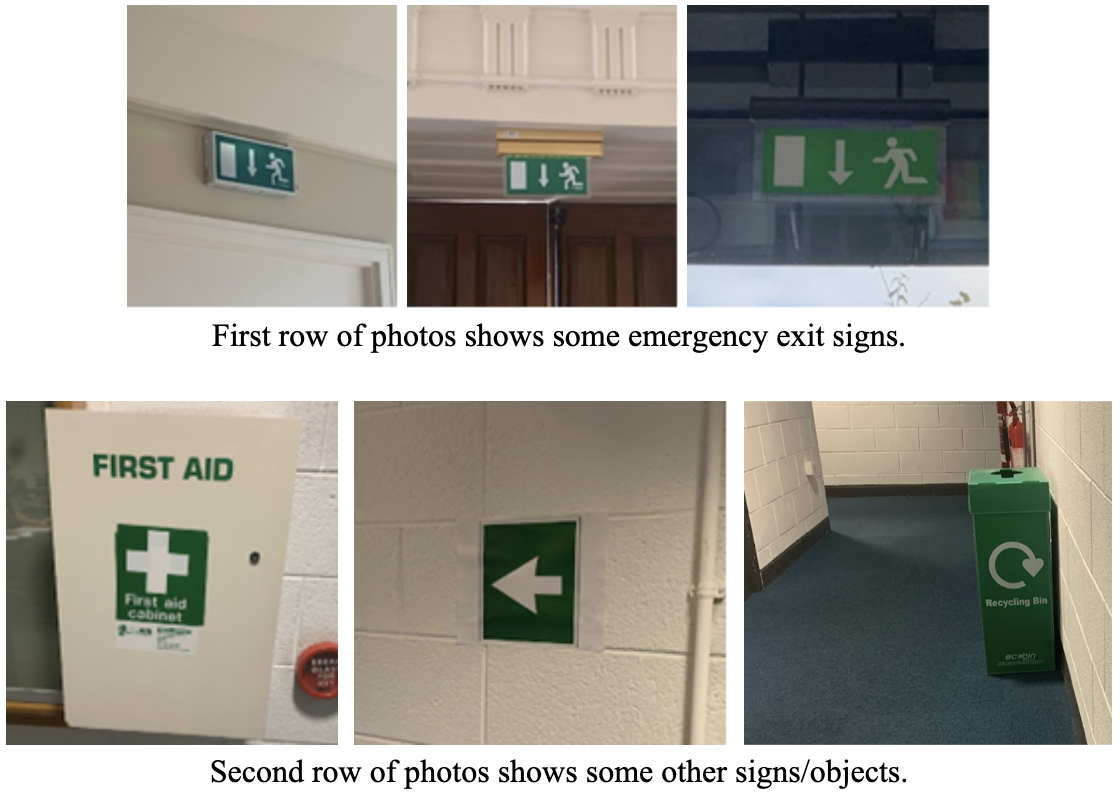
\includegraphics[width=0.75\textwidth]{q1a.png}
    \caption[1.(a)]{Question 1.(a) images}
    \label{fig:q1a-fig}
\end{figure}


1. (b) [COMPARE \& CONTRAST QUESTION] Compare and contrast: 
\begin{itemize}
    \item Non-Maxima Suppression as used in first derivative edge detection. 
    \item Non-Maxima Suppression as used in the first stage of SIFT. 
    \item Non-Maxima Suppression as used in Moravec corner detection. 
    \item Non-Maxima Suppression as used in the Hough transform for circles where the radius is unknown.  
\end{itemize}

You must provide a list of the differences and similarities between the techniques.   Each of the differences and similarities must be clearly explained.  NOTE:  Marks will only be awarded for the detailed comparison of techniques.  No marks will be awarded for separate descriptions of the techniques                    [25 marks] 
\end{document}

